\section{Coarsening for Elastostatics}
In this study, we introduce data-driven finite elements (DDFEM) to 
improve the simulation speed at the cost of small inaccuracy for elastostatic problems with heterogeneous non-linear materials. DDFEM focuses on finite elements defined one a regular grid.
To handle irregular boundary geometry, we will apply the use embedded finite elements for partially filled elements.
Using regular elements enables trivial combination of fine elements into coarser blocks of elements. This operation can be applied hierarchically to coarsen a mesh multiple times.
In this section, we discuss the two main stages of DDFEM computation---offline metamaterial construction and online coarsening.

\paragraph{Material palettes and mappings}
This study focuses on designs made of a discrete set of materials. The methodology can be extended to handle continuous mixtures of materials.
We note that designers often do not work in a continuous space of materials but limit themselves to a relatively compact set (e.g. rubber, wood, steel) related to their problem domain. We call these discrete sets of materials palettes and denote them $\set{P}=\{\material_0, \material_1, \hdots, \material_n\}$. Here $\material_i$ denotes a specific material model in $\set{P}$, and $n$ is the size of the material palette. In this work we further limit ourselves to (nonlinear) hyper-elastic materials, which means that each $\material_i$ can be represented by a strain energy density function $V$.
We also include a void (or empty) material in every palette. This allows us to perform topology changes in the same manner in which we perform material assignment updates.
In subsequent sections, we use a left superscript to indicate the level of coarsening. For example, $\set{P}^0$ denotes a material palette at the fine scale while $\set{P}^1$ denotes the new palette of metamaterials that results from the first coarsening step.

\paragraph{Coarsening for finite elements}
The key component of our DDFEM is coarsening. It reduces the number of elements in a finite element simulation mesh in order to improve runtime performance. Since simply removing elements can greatly reduce the accuracy of the simulation, coarsening schemes assign new materials to coarsened elements to minimize this effect.
We regard the global coarsening of a simulation mesh as the result of many local coarsening operations which map from contiguous subsets of fine elements with applied materials to coarse elements with new, optimized materials.
Our goal is to precompute these fitted materials so that coarsening is fast at runtime.

Each local coarsening operation merges a 2x2 block of elements into a single coarse element (Figure~\ref{fig:coarsen}).
\begin{figure}
	\centering
	
	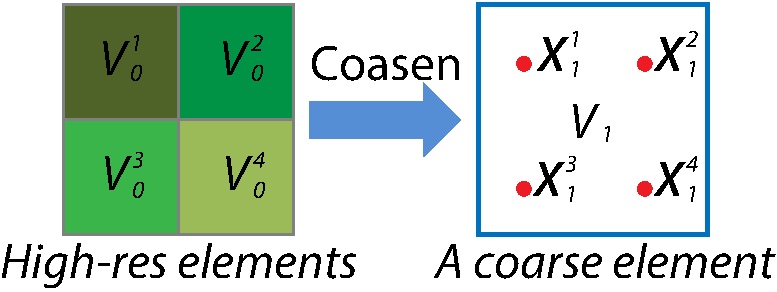
\includegraphics[width=0.5\textwidth]{images/coarsen.pdf}
	\caption{Coarsening a 2x2 block of }
	\label{fig:coarsen}
\end{figure}
\paragraph{Conforming vs.~embedded finite elements}
The defining feature of conforming finite element methods is that the simulation mesh is aligned with the geometry of the object being simulated. One obvious feature of conforming meshes is that the mesh itself is a function of the input geometry. This means that the output of a local coarsening operator (the coarsened mesh) will also be a function of the input geometry. Also, the new material computed by each local coarsening operator will be a function of input geometry. This dependence on input geometry is a significant issue to overcome if we wish to precompute coarsened materials because, in design problems, the input geometry is in constant flux. The number of precomputed coarse materials now depends on the local material assignment on the simulation mesh and the input geometry. Thus space of coarsened materials is prohibitively large. 
To mitigate this we turn to embedded finite elements. These methods embed the geometry to be simulated into the simulation mesh with no regard for whether the mesh conforms to the geometry or not. Thus an identical simulation mesh can be used for any input geometry. Local coarsening operations on the embedded mesh yield identical coarse elements and the optimized coarse material depends only on the local material distribution on the simulation mesh.  This significantly reduces the size of the coarsened material space. In this paper we embed all simulation geometry into a regular hexahedral mesh.

\paragraph{Algorithms}
With the material palette in hand, we can now define our algorithm, which is divided into two distinct phases: an \textbf{offline database construction} stage and an \textbf{online coarsening} stage.  Below we detail the input, output, and steps of each stage:

\begin{algorithm}
	\caption{Offline Database Construction}\label{alg:off}
	\begin{algorithmic}[1]
		\Procedure{DatabaseConstruction}{ }
		\State $^0\set{P}$: Input material palette
		\State $^1\set{P}$: new palatte of metamaterials
		\State $S\gets$ initial designs
		\State $A\gets \emptyset$
		\Do
		\State stochasticSampling($S$, $A$, $F$, $\mathcal{X}$)
		\State $\mathbf{s}_i\gets$ selectCandidate($S$)
		\State $\mathbf{d}\gets$ selectDirection($A$, $F$, $\mathcal{X}$)
		\State $\mathbf{x}_i \gets$ localOptimization($\mathbf{s}_i$, $\mathbf{d}$, ${F}$, $\mathcal{X}$)
		\State add $\mathbf{x}_i$ to $A$
		\If {$\mathbf{x}_i$ is dominated by $A$}
		\State \textbf{continue} 
		\Else
		\State $(M_i,\mathcal{U}_i)\gets $ localSearch($\mathbf{x}_i$, $A$, $F$, $\mathcal{X}$)
		\State add $(M_i,\mathcal{U}_i)$ to $A$
		\EndIf
		\doWhile within computation budget
		\State $P\gets$ dominatingHypersurfaces($A$)
		\State \Return $P$
		\EndProcedure
	\end{algorithmic}
\end{algorithm}

	\item \textbf{OUTPUT:} A new palette of coarse metamaterials, $^1\set{P}$, and a mapping from fine material combinations to the coarsened materials in $^1\set{P}$. 
	\item \textbf{FOR EACH} material combination applied to a 2$\times$2$\times$2 cube of high resolution elements
	\subitem $\bullet$ Sample potential energy function of 2$\times$2$\times$2 block
	\subitem $\bullet$ Fit metamaterial for coarse hexahedral element
	\subitem $\bullet$ Add metamaterial to $^1\set{P}$ using high resolution 
	\subitem material IDs as database key
	\item \textbf{END}
\end{itemize}
\hrule\\
\textbf{Online Coarsening}\\
\hrule \\~
\begin{itemize}
	\item \textbf{INPUT:} High resolution hexahedral simulation mesh with 
	\subitem material IDs and
	\subitem coarsened hexahedral simulation mesh 
	\item \textbf{OUTPUT:} Metamaterial assignments for coarse mesh
	\item \textbf{FOR EACH} 2$\times$2$\times$2 block in the high resolution mesh
	\subitem $\bullet$ Replace with single coarse element
	\subitem $\bullet$ Assign material from $^1\set{P}$ using high resolution 
	\subitem material IDs as database key 
	\item \textbf{END}
\end{itemize}
\hrule

\paragraph{Hierarchical coarsening}
We stress that both stages of the DDFEM algorithm can be applied hierarchically. Given the first level of metamaterials, $^1\set{P}$, we can construct a metamaterial library, $^2\set{P}$, for the second level by using $^1\set{P}$ as an input material palette. At runtime, the coarsening algorithm looks up materials from $^2\set{P}$ to replace each 2$\times$2$\times$2 coarse block with a single element.

Having introduced the broad strokes of the DDFEM scheme, we move on to a detailed explanation of each algorithmic component. First we discuss database construction in Section~\ref{sec:database}, followed by the runtime component in Section~\ref{sec:runtime}. We end by demonstrating the speed and accuracy of DDFEM in Section~\ref{sec:result}.